\documentclass[../main.tex]{subfiles}

\begin{document}

We now examine the reduction in sample impoverishment due to the dense sampling improvement described in \autoref{sec:inference_RBPF}. 

Similarly to \autoref{sec:inference_RBPF}, we demonstrate the problem of sample impoverishment by simulating a single time step of the particle filter, for varying values of $\vt$. Fixing $\mu_k^{(i)}$, $\Sigma_k^{(i)}$ whilst varying $y_k$ and $N$, we simulate one time step of the RBPF update step described above and present the normalised entropy of the RBPF particle weights with and without the dense sampling improvement in Figure \ref{fig:2__2__2__sample_impoverishment}.

\begin{figure}[h!]
	\centering
	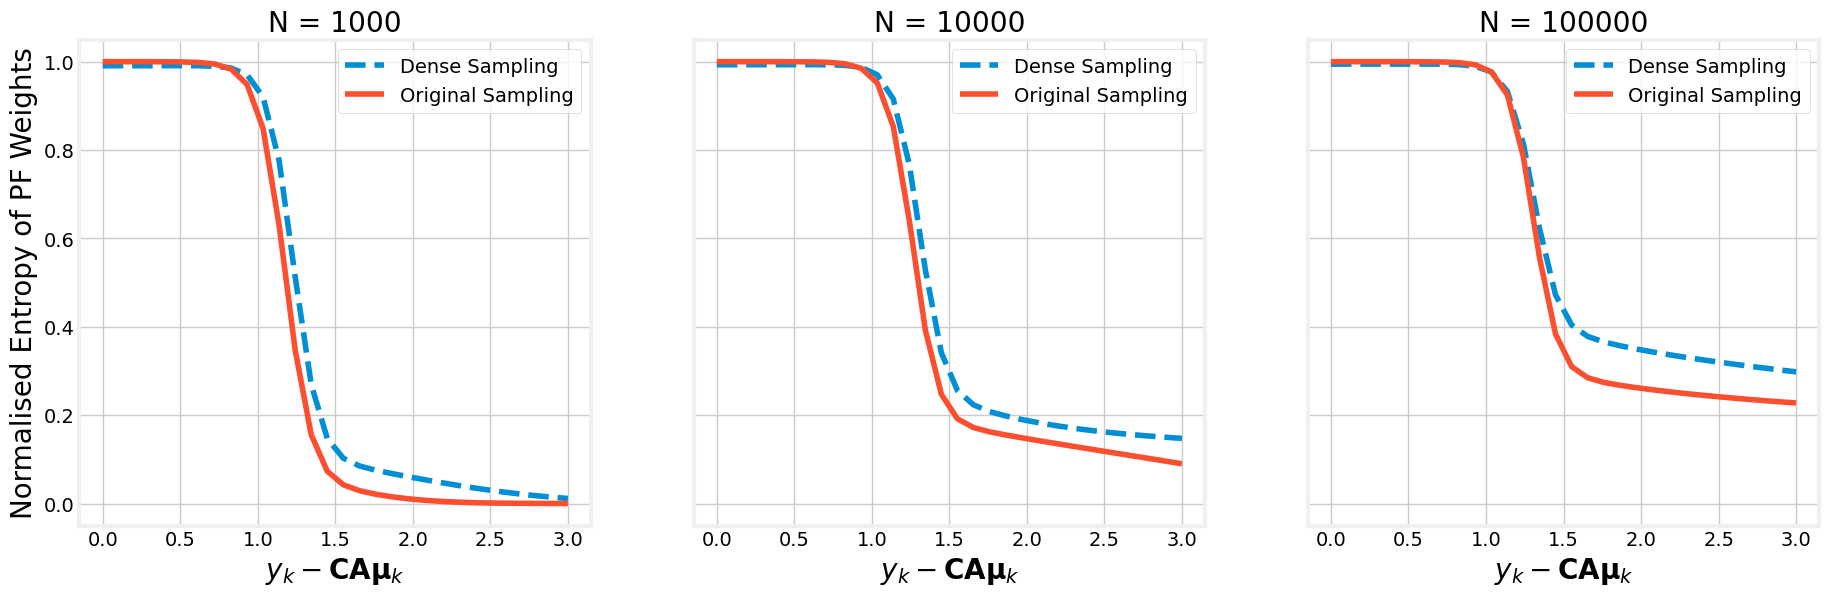
\includegraphics[width=15.0cm]{../plots/4__1__1__dense_sampling.png}
	\caption{Improvement in normalised entropy of RBPF particle weights using dense sampling with hyperparameters: ($\epsilon_\lambda = 0.1$, $m=2$)}
	\label{fig:4__1__1__dense_sampling}
\end{figure}	

We can see from Figure \ref{fig:2__2__2__sample_impoverishment} that the dense sampling improvement causes the normalised entropy of the RBPF particle weights to increase for larger price outliers $\vt$. A higher normalised entropy indicates that the weights of the RBPF particles are more evenly distributed and hence that there are a larger number of particles with effective weights under the dense sampling improvement. This helps to reduce sample impoverishment, and can improve the performance of the generic RBPF. 
	
\end{document}